
% !TeX spellcheck = en

\chapter{Database Change Scenarios}
This section shows how to handle the predefined scenarios for the given change management tool. This includes following scenarios: 

\begin{itemize}
	\item Rename an attribute.
	\item Add an attribute and set the value as a constant.
	\item Delete an attribute.
	\item Change an attribute type and add an SQL script to fill it from existing values.
	\item Rename a table and change a related view which uses this table.
	\item Split a column into two columns
\end{itemize}

The changes were applied to an existing database Pagila \cite{Hillyer}. Each first two migrations are to setup the database, first the create the schema and second to insert the specific data.

\section{Flyway Scenarios}

\subsection{Using CLI}
\marginpar{Setup \cite{FlywayGetStarted}}%
To create a first migration, add a database change as sql file into the sql directory (see \autoref{fig:flyway_folder_structure}). 
The scripts \texttt{V1\_\_create\_db.sql} and \texttt{V2\_\_insert\_pagila\_data.sql} set up the pagila database as illustrated in \autoref{fig:flyway_empty_db}. When running  \texttt{flyway migrate}, flyway wants to adapt the schema history table. But as this table does not exist, it will create a new one instead.


 

\begin{figure}[H]
	\centering
	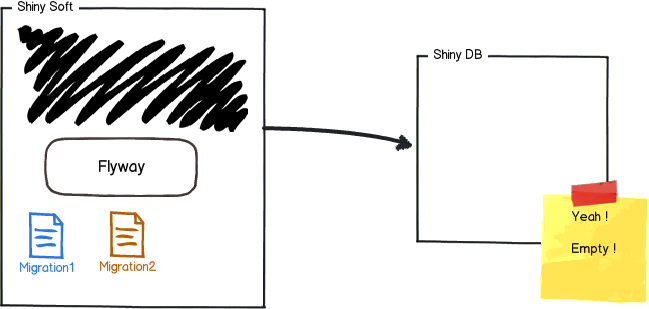
\includegraphics[width=0.45\textwidth]{./chapters/scenarios/images/EmptyDb}
	\caption[Flyway empty database - Source: \cite{FlywayGetStarted}]{Flyway empty database}
	 \label{fig:flyway_empty_db}
\end{figure}
Now the table \textit{flyway\_schema\_history} has been created via the first flyway migration. This metadata table holds various information regarding the database migrations and their history. After this initialization, flyway runs the migration scripts in the sql directory according on their version number subsequently. 
BASELINE MODEL! To start with a baseline

\begin{figure}[H]
	\centering
	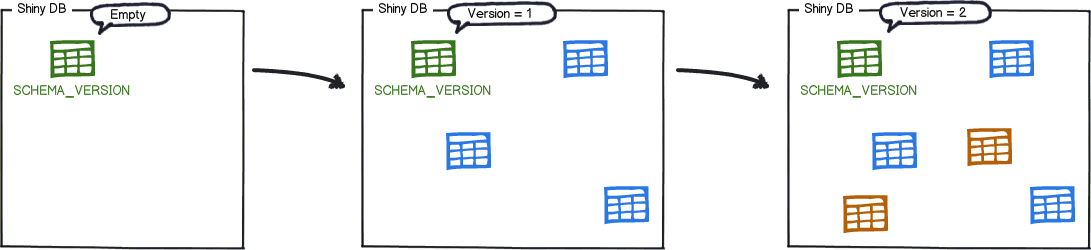
\includegraphics[width=0.85\textwidth]{./chapters/scenarios/images/Migration-1-2}
	\caption[Flyway first migrations - Source: \cite{FlywayGetStarted}]{Flyway first migrations}
	\label{fig:Migration-1-2}
\end{figure}

\textbf{Scenario 1: Rename an Attribute}\\
\marginpar{Scenario 1}%
The first change specific migration is in the sql migration script\\ \texttt{V3\_\_rename\_attribute.sql}:
\begin{lstlisting}[language=SQL]
ALTER TABLE customer RENAME COLUMN email TO private_email;
\end{lstlisting}
After just adding the script to de sql directory, flyway already knows the change and stores it into the meta data table. With \texttt{flyway info} the migration status can be asked:

\begin{figure}[H]
	\centering
	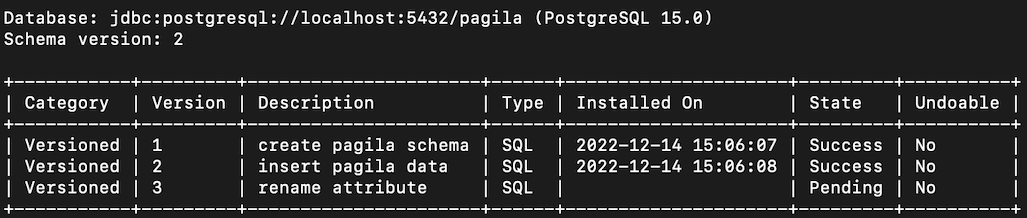
\includegraphics[width=0.95\textwidth]{./chapters/scenarios/images/flyway_metadata_v2}
	\caption[Flyway meta data table - Source: Own illustration]{Flyway meta data table}
	% \label{fig:bsp_chapter:example_figure}
\end{figure}
In order to perform the migration effectively, the command \texttt{flyway migrate} is applied.



\textbf{Scenario 2: Add an Attribute and Set the Value as a Constant}\\
\marginpar{Scenario 2}%
To apply the second migration the following script is applied in V3.
\begin{lstlisting}[language=SQL]
ALTER TABLE customer ADD COLUMN gender VARCHAR(50);

UPDATE customer
SET gender = 'undefined';
\end{lstlisting}
Flyway generates a checksum for every applied migration. This checksum is used to track if a file was changes after its applied migration. If such a change occurs, a new migration will cause an error and asks to either revert the change or to run \texttt{flyway repair} to update the schema history.
If a developer would change the default value of gender from \textit{undefined} to \textit{undef} and run a new migration, it would fail. To fix this run \texttt{flyway repair}. Even the environment is now fixed, the change gender equals \textit{undef} is not applied and still \textit{undefined}.


\textbf{Scenario 3: Delete an Attribute}\\
\marginpar{Scenario 3}%

\begin{lstlisting}[language=SQL]
ALTER TABLE customer
DROP COLUMN gender;
\end{lstlisting}


\textbf{Scenario 4: Change an Attribute Type and Add an SQL Script to Fill from Existing Values}\\
\marginpar{Scenario 4}%
To change an attribute type the migration in the file \texttt{V6\_\_change\_attribute\_type.sql} was applied with flyway migrate:
\begin{lstlisting}[language=SQL]
ALTER TABLE customer
ALTER COLUMN private_email TYPE VARCHAR(100) USING private_email::varchar;
\end{lstlisting}


\textbf{Scenario 5: Rename a Table and Change a Related View which uses this Table}\\
\marginpar{Scenario 5}%
The next migration is to change a related view after renaming a table\\
\texttt{V7\_\_change\_attribute\_type.sql} was applied with flyway migrate:
\begin{lstlisting}[language=SQL]
ALTER TABLE customer RENAME TO clients;
	
	
CREATE OR REPLACE VIEW customer_list AS
SELECT cl.customer_id AS id,
	(cl.first_name || ' '::text) || cl.last_name AS name,
	a.address,
	a.postal_code AS "zip code",
	a.phone,
	city.city,
	country.country,
	CASE
		WHEN cl.activebool THEN 'active'::text
		ELSE ''::text
	END AS notes,
	cl.store_id AS sid
FROM clients cl
JOIN address a ON cl.address_id = a.address_id
JOIN city ON a.city_id = city.city_id
JOIN country ON city.country_id = country.country_id;
\end{lstlisting}

After this second to last migration the flyway schema history looks like the following:
\begin{figure}[H]
	\centering
	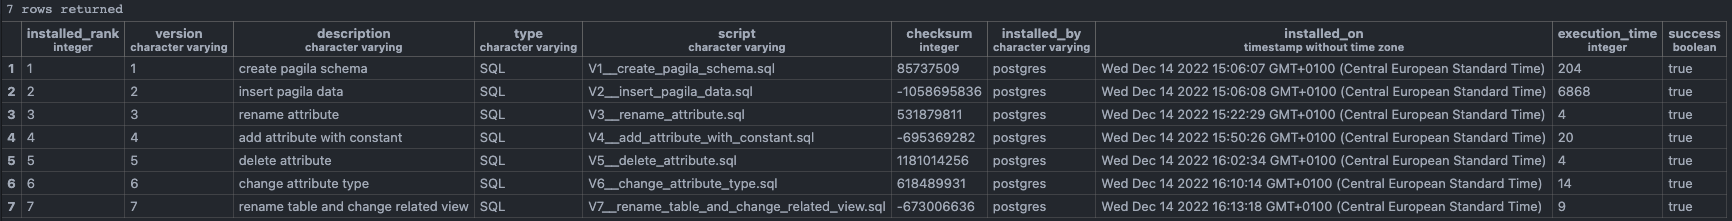
\includegraphics[width=1.1\textwidth]{./chapters/scenarios/images/flyway_schema_history}
	\caption[Flyway Schema History - Source: Own illustration]{Flyway Schema History}
	% \label{fig:bsp_chapter:example_figure}
\end{figure}
For every migration the date inclusive time, the script or the user that applied the script is stored.

\newpage
\textbf{Scenario 6: Split an Attribute into two Attributes}\\
\marginpar{Scenario 6}%
First two new columns are created and then the string is split and distributed into the two new columns.

\begin{lstlisting}[language=SQL]
ALTER TABLE address ADD COLUMN street text;
ALTER TABLE address ADD COLUMN house_number text;


WITH results AS (
	SELECT address_id as id,
	(string_to_array(address, ' '))[1] as a1,
	array_to_string((string_to_array(address, ' '))[2:], ' ') as a2
	from address
)

UPDATE address
SET house_number = (SELECT a1 FROM results WHERE address_id = results.id),
street = (SELECT a2 FROM results WHERE address_id = results.id);
\end{lstlisting}

All migrations could be implemented in PostgreSQL and executed without any problems. There were no limitations or problems with any of the migrations.


\marginpar{Failed\\ migration \cite{Lukonin2017}}%
Flyway automatically wraps every migration script in a transaction, which allows for automatic rollback in case of an error. If your database supports DDL transactions (such as PostgreSQL), the entire migration script will be rolled back automatically. However, if you are using SQL Server, the DDL queries will be committed automatically, so you will need to create manual rollback scripts or use idempotent scripts to roll back the changes. If your migration script does not contain DDL commands, it will generally be automatically rolled back by most database engines in case of an error.\\
To make the rollback process easier, Flyway supports rollback scripts, which can be created for every versioned migration file using the naming convention \textit{U\#\#\#\_\_text.sql}. If a migration fails, Flyway will automatically run the corresponding rollback script. The UNDO command (see \autoref{flyway_features}) can also be used to manually trigger a rollback, which will roll back the latest migration by default. Alternatively, taking a snapshot of the database before release and restoring it if any migration goes wrong is the cleanest approach, but may not always be feasible. It is important to have a well-designed rollback strategy in place, which may involve creating proper rollback scripts and using idempotent migrations to make the process easier.

\newpage
\subsection{Usage with Java API}
\marginpar{Java Migration}%
Flyway is most useful when integrated into an application. By doing so, the compatibility between the application and its database can be maintained automatically, without the need for manual intervention. Flyway checks the version of the database and automatically applies new migrations before the rest of the application begins. This is crucial because the database must be in a state that is compatible with the rest of the code before the application can function properly. Hereby flyway can use migration files written in classic SQL in the directory \textit{src/main/resources/db.migration/}, similar to the last chapter.

\begin{lstlisting}[language=Java]
import org.flywaydb.core.Flyway;

public class App {
	public static void main(String[] args) {
		// Create the Flyway instance and point it to the database
		Flyway flyway = Flyway.configure().dataSource("jdbc:h2:file:./target/foobar", "sa", null).load();
		flyway.migrate(); // Start the migration
	}
}
\end{lstlisting}

\marginpar{Java Migration}%
Another option is to implement the migrations directly as a Java class. Running Flyway through the API on application startup is the most efficient and reliable method. This method allows you to combine all migrations with your application, making it easy to deploy to any environment. The API will automatically detect the state of the database and perform the necessary migrations on startup, ensuring that your application code is always compatible with the database it is accessing.
Flyway can be integrated in Gradle or Maven as in the following example.

%\begin{lstlisting}[language=Java, caption={File: src/main/java/db/migration/V1\_\_create_\pagila\_schema.sql}]
\begin{lstlisting}[language=Java, caption={File: src/main/java/db/migration/V3\_\_rename\_attribute.sql}]
package db.migration;

import org.flywaydb.core.api.migration.BaseJavaMigration;
import org.flywaydb.core.api.migration.Context;
import java.sql.PreparedStatement;

public class V1__RenameAttribute extends BaseJavaMigration {
	public void migrate(Context context) throws Exception {
		try {
			PreparedStatement statement = context.getConnection().prepareStatement("ALTER TABLE customer RENAME COLUMN email TO private_email;")) {
						statement.execute();
			}
	}
}
\end{lstlisting}

With the command below the migration can be applied.
 \begin{lstlisting}
mvn flyway:migrate
 \end{lstlisting}


\newpage
\section{Liquibase Scenarios}
\marginpar{Information \cite{Liquibase}}%
The first changeset applied on the database will automatically create the databasechangelog and the databasechangeloglock table. 

\begin{figure}[H]
	\centering
	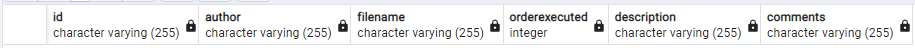
\includegraphics[width=\textwidth]{./chapters/scenarios/images/databasechangelog}
	\caption[DatabaseChangeLog Table - Source: Own illustration]{DatabaseChangeLog Table}
	\label{fig:scenarios:LiquibaseDBCL}
\end{figure}

\begin{figure}[H]
	\centering
	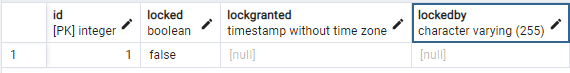
\includegraphics[width=0.8\textwidth]{./chapters/scenarios/images/databasechangeloglock}
	\caption[DatabaseChangeLogLock Table - Source: Own illustration]{DatabaseChangeLogLock Table}
	\label{fig:scenarios:LiquibaseDBCLL}
\end{figure}


\subsection{SQL-Changelog}
\marginpar{SQL-Changelog \cite{Liquibase}}%
SQL changelogs always start with a comment specifying the format of SQL. In addition, each changeset starts with a comment specifying the author and attributes. The attributes either add additional information like a label or add additional functionality to the changeset. Please refer to the Liquibase documentation \cite{Liquibase} for a complete list of possible attributes. The changeset contains the changes as SQL statements and can be expanded by the comment or rollback statement. SQL changelogs do not support automatic rollback, so each changeset needs a defined rollback statement to use this feature.

\begin{lstlisting}[language=SQL, caption={SQL Changelog with Example Changeset}, label=list:scenarios:LiquibaseSQLChangesetExample]
	--liquibase formatted sql
	
	--changeset author:id attribute1:value1 attribute2:value2
	-- comment: Describe the Change
	
	SQL STATEMENT
	
	-- rollback SQL STATEMENT
\end{lstlisting}

\textbf{Scenario 1: Rename an Attribute}\\
\marginpar{Scenario 1}%
\begin{lstlisting}[language=SQL, caption={SQL Changeset Scenario 1: Rename an Attribute}, label=list:scenarions:LiquibaseSQLScen1]
	--changeset C.Kleinstein:1 labels:Scenario 1 
	--comment: Scenario 1, Renaming an Attribute
	
	ALTER TABLE customer RENAME COLUMN email TO private_email;
	
	--rollback ALTER TABLE customer RENAME COLUMN private_email TO email;
\end{lstlisting}

\textbf{Scenario 2: Add an Attribute and Set the Value as a Constant}\\
\marginpar{Scenario 2}%
\begin{lstlisting}[language=SQL, caption={SQL Changeset Scenario 2: Add an Attribute and Set the Value as a Constant}, label=list:scenarions:LiquibaseSQLScen2]
	--changeset C.Kleinstein:2 labels:Scenario 2
	--comment: Scenario 2, Add Attribute and fill with const Value
	
	ALTER TABLE customer ADD COLUMN gender VARCHAR(50);
	
	UPDATE customer SET gender = 'undefined';
	
	--rollback ALTER TABLE customer DROP COLUMN gender;
\end{lstlisting}

\textbf{Scenario 3: Delete an Attribute}\\
\marginpar{Scenario 3}%
\begin{lstlisting}[language=SQL, caption={SQL Changeset Scenario 3: Delete an Attribute}, label=list:scenarions:LiquibaseSQLScen3]
	--changeset C.Kleinstein:3 labels:Scenario 3
	--comment: Scenario 3, Delete an Attribute
	
	ALTER TABLE customer DROP COLUMN gender;
	
	--rollback ALTER TABLE customer ADD COLUMN gender VARCHAR(50);
\end{lstlisting}

\textbf{Scenario 4: Change an Attribute Type and Add an SQL Script to Fill from Existing Values}\\
\marginpar{Scenario 4}%
\begin{lstlisting}[language=SQL, caption={SQL Changeset Scenario 4: Change an Attribute Type and Add an SQL Script to Fill from Existing Values}, label=list:scenarions:LiquibaseSQLScen4]
	--changeset C.Kleinstein:4 labels:Scenario 4
	--comment: Scenario 4, Change Attribute type
	
	ALTER TABLE customer ALTER COLUMN private_email TYPE VARCHAR(100) USING private_email::varchar;
	
	--rollback ALTER TABLE customer ALTER COLUMN private_email TYPE TEXT USING private_email::text;
\end{lstlisting}

\newpage
\textbf{Scenario 5: Rename a Table and Change a Related View which uses this Table}\\
\marginpar{Scenario 5}%
\begin{lstlisting}[language=SQL, caption={SQL Changeset Scenario 5: Rename a Table and Change a Related View which uses this Table}, label=list:scenarions:LiquibaseSQLScen5]
--changeset C.Kleinstein:5 labels:Scenario 5 
--comment: Scenario 5, Rename a table with a related view

	ALTER TABLE customer RENAME TO clients;
	CREATE OR REPLACE VIEW customer_list
	AS
	SELECT cl.customer_id AS id,
		(cl.first_name || ' '::text) || cl.last_name AS name,
		a.address,
		a.postal_code AS "zip code",
		a.phone,
		city.city,
		country.country,
			CASE
				WHEN cl.activebool THEN 'active'::text
				ELSE ''::text
			END AS notes,
		cl.store_id AS sid
	FROM clients cl
		JOIN address a ON cl.address_id = a.address_id
		JOIN city ON a.city_id = city.city_id
		JOIN country ON city.country_id = country.country_id;
	
	--rollback ALTER TABLE clients RENAME TO customer; 
	--rollback CREATE OR REPLACE VIEW customer_list
	--rollback AS
	--rollback SELECT cu.customer_id AS id,
	--rollback (cu.first_name || ' '::text) || cu.last_name AS name,
	--rollback     a.address,
	--rollback     a.postal_code AS "zip code",
	--rollback     a.phone,
	--rollback     city.city,
	--rollback     country.country,
	--rollback         CASE
	--rollback             WHEN cu.activebool THEN 'active'::text
	--rollback             ELSE ''::text
	--rollback         END AS notes,
	--rollback     cu.store_id AS sid
	--rollback FROM customer cu
	--rollback      JOIN address a ON cu.address_id = a.address_id
	--rollback      JOIN city ON a.city_id = city.city_id
	--rollback      JOIN country ON city.country_id = country.country_id;
\end{lstlisting}

\newpage
\textbf{Scenario 6: Split an Attribute into two Attributes}\\
\marginpar{Scenario 6}%
\begin{lstlisting}[language=SQL, caption={SQL Changeset Scenario 6: Split an Attribute into two Attributes}, label=list:scenarions:LiquibaseSQLScen6]
--changeset C.Kleinstein:6 labels:Scenario 6
--comment: Scenario 6, Split one Attribute into two

	ALTER TABLE address ADD COLUMN house_number text;
	ALTER TABLE address ADD COLUMN street text;
	
	WITH results AS (
		SELECT address_id as id,
		(string_to_array(address, ' '))[1] as a1,
		array_to_string((string_to_array(address, ' '))[2:], ' ') as a2
	from address
	)
	UPDATE address
	SET house_number = (SELECT a1 FROM results WHERE address_id = results.id),
	street = (SELECT a2 FROM results WHERE address_id = results.id);
	
	--rollback ALTER TABLE address DROP COLUMN house_number;
	--rollback ALTER TABLE address DROP COLUMN street;
\end{lstlisting}

\textbf{DatabaseChagneLog Table}\\
\marginpar{DatabaseChagneLog Table}%
Figure \ref{fig:scenarios:LiquibaseDBCLSQL} shows the database changelog after all six changesets have been applied.

\begin{figure}[H]
	\centering
	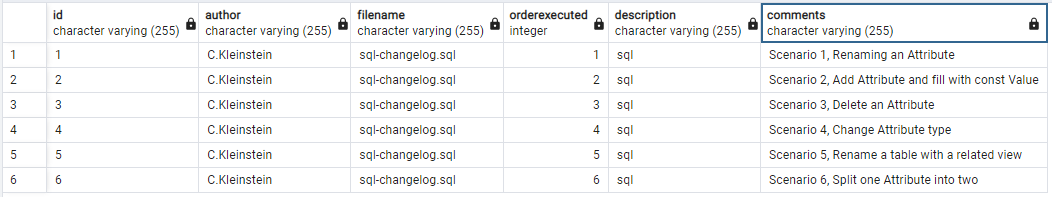
\includegraphics[width=\textwidth]{./chapters/scenarios/images/databasechangelogSQL}
	\caption[DatabaseChangeLog Table - Source: Own illustration]{DatabaseChangeLog Table}
	\label{fig:scenarios:LiquibaseDBCLSQL}
\end{figure}

\subsection{YAML-Changelog}
\marginpar{YAML-Changelog \cite{Liquibase}}%
The YAML changelog defines changesets consisting of different change types. The change type defines the change and is database independent. However, the change types available from Liquibase cannot cover all changes typically done on databases. Furthermore, not all change types provide an automatic rollback that needs to be explicitly defined by the user.
\newpage

\begin{lstlisting}[language=SQL, caption={YAML Changelog with Example Changeset}, label=list:scenarios:LiquibaseYAMLChangesetExample]
databaseChangeLog:  

-  changeSet:  
	id:  1  
	author:  Author 
	changes:  
	-  ChangeType1:
		attribute1: value1
		
	rollback:  
	- ChangeType2:
		attribute2: value2
 
\end{lstlisting}

\textbf{Scenario 1: Rename an Attribute}\\
\marginpar{Scenario 1}%
\begin{lstlisting}[language=SQL, caption={YAML Changeset Scenario 1: Rename an Attribute}, label=list:scenarions:LiquibaseYAMLScen1]
databaseChangeLog:
- changeSet:  
	id:  1  
	author:  C.Kleinstein  
	changes:  
	-  renameColumn:  
		catalogName:  customer  
		columnDataType:  text  
		newColumnName:  private_email  
		oldColumnName:  email  
		schemaName:  public  
		tableName:  customer
\end{lstlisting}

\textbf{Scenario 2: Add an Attribute and Set the Value as a Constant}\\
\marginpar{Scenario 2}%
\begin{lstlisting}[language=SQL, caption={YAML Changeset Scenario 2: Add an Attribute and Set the Value as a Constant}, label=list:scenarions:LiquibaseYAMLScen2]
- changeSet: 
	id:  2
	author: C.Kleinstein
	changes:
	- addColumn:
		tableName: customer
		columns:
		- column:
			name: gender
			type: varchar(50)
			value: undefined
\end{lstlisting}

\textbf{Scenario 3: Delete an Attribute}\\
\marginpar{Scenario 3}%
The \texttt{dropColumn} changetype does not support auto rollback. The rollback needs to explicitly designed.
\begin{lstlisting}[language=SQL, caption={SQL Changeset Scenario 3: Delete an Attribute}, label=list:scenarions:LiquibaseSQLScen3]
- changeSet: 
	id:  3
	author: C.Kleinstein
	changes:
		- dropColumn:
		tableName: customer
		columns:
		- column:
			name: gender
	rollback:
        - addColumn:
			tableName: customer
			columns:
			- column:
				name: gender
				type: varchar(50)
				value: undefined
\end{lstlisting}

\textbf{Scenario 4: Change an Attribute Type and Add an SQL Script to Fill from Existing Values}\\
\marginpar{Scenario 4}%
The \texttt{modifyDataType} changetype does not support auto rollback. The rollback needs to explicitly designed.
\begin{lstlisting}[language=SQL, caption={SQL Changeset Scenario 4: Change an Attribute Type and Add an SQL Script to Fill from Existing Values}, label=list:scenarions:LiquibaseSQLScen4]
- changeSet:
	id: 4
	author: C.Kleinstein
	changes:  
	-  modifyDataType:    
		columnName:  private_email  
		newDataType:  varchar(100)    
		tableName:  customer
	rollback:
    -  modifyDataType:    
		columnName:  private_email  
		newDataType:  varchar(100)    
		tableName:  customer
\end{lstlisting}

\newpage
\textbf{Scenario 5: Rename a Table and Change a Related View which uses this Table}\\
\marginpar{Scenario 5}%
This scenario is not supported by Liquibase's change types and needs to be defined directly with SQL. Furthermore, by using SQL we also need to define a rollback as they are not supported with SQL.
\begin{lstlisting}[language=SQL, caption={SQL Changeset Scenario 5: Rename a Table and Change a Related View which uses this Table}, label=list:scenarions:LiquibaseSQLScen5]
- changeSet:
	id: 5
	author: C.Kleinstein
	changes:  
	-  renameTable:   
		newTableName:  clients  
		oldTableName:  customer 
	-  createView:         
	replaceIfExists:  true    
	selectQuery:  	SELECT cl.customer_id AS id,
						(cl.first_name || ' '::text) || cl.last_name AS name,
						a.address,
						a.postal_code AS "zip code",
						a.phone,
						city.city,
						country.country,
							CASE
								WHEN cl.activebool THEN 'active'::text
								ELSE ''::text
							END AS notes,
						cl.store_id AS sid
					FROM clients cl
						JOIN address a ON cl.address_id = a.address_id
						JOIN city ON a.city_id = city.city_id
						JOIN country ON city.country_id = country.country_id;
	viewName:  customer_list
	rollback:
		- sql:
			sql: 	ALTER TABLE clients RENAME TO customer; 
					CREATE OR REPLACE VIEW customer_list
					AS
					SELECT cu.customer_id AS id,
						(cu.first_name || ' '::text) || cu.last_name AS name,
						a.address,
						a.postal_code AS "zip code",
						a.phone,
						city.city,
						country.country,
							CASE
								WHEN cu.activebool THEN 'active'::text
								ELSE ''::text
							END AS notes,
						cu.store_id AS sid
					FROM customer cu
						JOIN address a ON cu.address_id = a.address_id
						JOIN city ON a.city_id = city.city_id
						JOIN country ON city.country_id = country.country_id;

\end{lstlisting}

\newpage
\textbf{Scenario 6: Split an Attribute into two Attributes}\\
\marginpar{Scenario 6}%
This scenario is not supported by Liquibase's change types and needs to be defined directly with SQL. Furthermore, by using SQL we also need to define a rollback as they are not supported with SQL.
\begin{lstlisting}[language=SQL, caption={SQL Changeset Scenario 6: Split an Attribute into two Attributes}, label=list:scenarions:LiquibaseSQLScen6]
- changeSet:
id: 6
author: C.Kleinstein
changes:
-  sql:
sql: 	ALTER TABLE address ADD COLUMN house_number text; 
		ALTER TABLE address ADD COLUMN street text; 
		WITH results AS (
			SELECT address_id as id,
			(string_to_array(address, ' '))[1] as a1,
			array_to_string((string_to_array(address, ' '))[2:], ' ') as a2
			from address) 
			
		UPDATE address 
		SET house_number = (SELECT a1 FROM results WHERE address_id = results.id), street = (SELECT a2 FROM results WHERE address_id = results.id);
rollback:
- sql:
sql:	ALTER TABLE address DROP COLUMN house_number; 
		ALTER TABLE address DROP COLUMN street;
\end{lstlisting}

\textbf{DatabaseChagneLog Table}\\
\marginpar{DatabaseChagneLog Table}%
Figure \ref{fig:scenarios:LiquibaseDBCLYAML} shows the database changelog after all six changesets have been applied.

\begin{figure}[H]
	\centering
	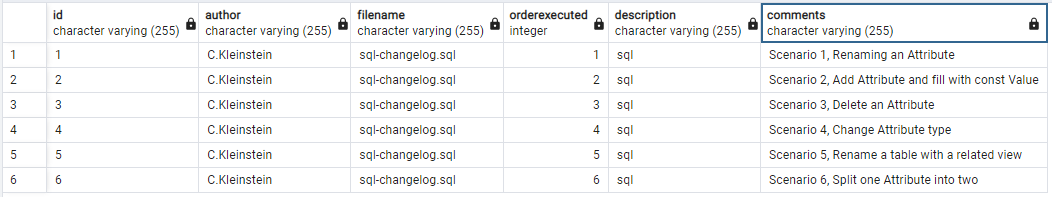
\includegraphics[width=\textwidth]{./chapters/scenarios/images/databasechangelogSQL}
	\caption[DatabaseChangeLog Table - Source: Own illustration]{DatabaseChangeLog Table}
	\label{fig:scenarios:LiquibaseDBCLYAML}
\end{figure}

\newpage